
% Define what kind of document we're going to write.
\documentclass[twocolumn]{article}

% For including images.
\usepackage{graphics}

% For including encapsulated postscript files.
\usepackage{epsfig}

% Needed to use the geometry command.
\usepackage{geometry}

% Set the size of the paper and the margins.
\geometry{letterpaper, portrait, margin=0.5in}

% Distance between columns.
\setlength{\columnsep}{0.4in}

% The package for the bibliography.
\usepackage{biblatex}

% The name of the bibliography file.
\addbibresource{references.bib}

% Set the title.
\title{\LARGE \bf My Paper Title}

% Set the author.
\author{Your Name Here}

% Start of the document.
\begin{document}

% Make the title
\maketitle

% Start of the abstract.
\begin{abstract}

All work and no play makes Jack a dull boy.
All work and no play makes Jack a dull boy.
All work and no play makes Jack a dull boy.
All work and no play makes Jack a dull boy.

All work and no play makes Jack a dull boy.
All work and no play makes Jack a dull boy.
All work and no play makes Jack a dull boy.
All work and no play makes Jack a dull boy.

% End of the abstract.
\end{abstract}

% New section.
\section{Introduction}
\label{sec:introduction}

All work and no play makes Jack a dull boy.
All work and no play makes Jack a dull boy.
\cite{knuthwebsite}
All work and no play makes Jack a dull boy.

All work and no play makes Jack a dull boy.
All work and no play makes Jack a dull boy.
All work and no play makes Jack a dull boy.

% New section.
\section{Details}
\label{sec:details}

All work and no play makes Jack a dull boy.
All work and no play makes Jack a dull boy.
All work and no play makes Jack a dull boy.

All work and no play makes Jack a dull boy.
All work and no play makes Jack a dull boy.
All work and no play makes Jack a dull boy.

% New sub-section.
\subsection{Figures}
\label{sec:details_figures}

Good, then we will shall fight in the shade.
Good, then we will shall fight in the shade.
Good, then we will shall fight in the shade.
Good, then we will shall fight in the shade.

% A figure.
\begin{figure}[h]
\centering
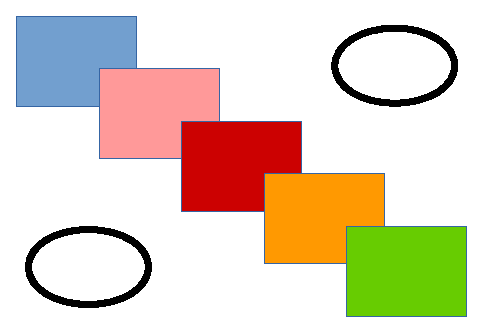
\includegraphics{../figures/shapes.eps}
\caption{These are some shapes.}
\label{fig:shapes}
\end{figure}

Good, then we will shall fight in the shade.
Good, then we will shall fight in the shade.
Good, then we will shall fight in the shade.
Good, then we will shall fight in the shade.

All work and no play makes Jack a dull boy.
All work and no play makes Jack a dull boy.
All work and no play makes Jack a dull boy.
All work and no play makes Jack a dull boy.

% A figure.
\begin{figure}[h]
\centering
\includegraphics[width=\linewidth,natwidth=400,natheight=300]{../figures/mountains.jpg}
\caption{Majestic mountains.}
\label{fig:mountains}
\end{figure}

% New sub-section.
\subsection{Bullets}
\label{sec:details_bullets}

% Start some bullets.
\begin{itemize}

\item All work and no play makes Jack a dull boy.
All work and no play makes Jack a dull boy.

\item All work and no play makes Jack a dull boy.
All work and no play makes Jack a dull boy.

% End the bullets.
\end{itemize}

% New sub-section.
\subsection{Equations}
\label{sec:details_equations}

All work and no play makes Jack a dull boy.

$$
\alpha + \beta = \chi \eqno{(1)}
$$

% New sub-section.
\subsection{Tables}
\label{sec:details_tables}

All work and no play makes Jack a dull boy.
All work and no play makes Jack a dull boy.
All work and no play makes Jack a dull boy.
All work and no play makes Jack a dull boy.

All work and no play makes Jack a dull boy.
All work and no play makes Jack a dull boy.
All work and no play makes Jack a dull boy.
All work and no play makes Jack a dull boy.

\begin{table}[h]
\caption{An Example of a Table}
\label{tab:table_a}
\begin{center}
\begin{tabular}{|c||c|c|}
\hline
One & Two & Three\\
\hline
Four & Five & Six\\
\hline
\end{tabular}
\end{center}
\end{table}

\section{Conclusion}
\label{sec:conclusions}

All work and no play makes Jack a dull boy.
All work and no play makes Jack a dull boy.
All work and no play makes Jack a dull boy.
All work and no play makes Jack a dull boy.

All work and no play makes Jack a dull boy.
All work and no play makes Jack a dull boy.
All work and no play makes Jack a dull boy.
All work and no play makes Jack a dull boy.

% New sub-section.
\subsection{Important Stuff}
\label{sec:conclusions_important_stuff}

All work and no play makes Jack a dull boy.
All work and no play makes Jack a dull boy.
All work and no play makes Jack a dull boy.
All work and no play makes Jack a dull boy.

\section*{Appendix}
\label{sec:appendix}

All work and no play makes Jack a dull boy.
All work and no play makes Jack a dull boy.
All work and no play makes Jack a dull boy.
All work and no play makes Jack a dull boy.

\section*{Acknowledgment}
\label{sec:acknowledgment}

All work and no play makes Jack a dull boy.
All work and no play makes Jack a dull boy.
All work and no play makes Jack a dull boy.
All work and no play makes Jack a dull boy.

% Generate the bibliography.
\printbibliography

% % Start of the bibliography.
% \begin{thebibliography}{99}

% \bibitem{c1} G. O. Young, Synthetic structure of industrial plastics (Book style with paper title and editor),   in Plastics, 2nd ed. vol. 3, J. Peters, Ed.  New York: McGraw-Hill, 1964, pp. 15Ð64.

% \bibitem{c2} W.-K. Chen, Linear Networks and Systems (Book style).  Belmont, CA: Wadsworth, 1993, pp. 123Ð135.

% \bibitem{c3} H. Poor, An Introduction to Signal Detection and Estimation.   New York: Springer-Verlag, 1985, ch. 4.

% \bibitem{c4} B. Smith, An approach to graphs of linear forms (Unpublished work style), unpublished.

% \bibitem{c5} E. H. Miller, A note on reflector arrays (Periodical styleÑAccepted for publication), IEEE Trans. Antennas Propagat., to be publised.

% % End of the bibliography.
% \end{thebibliography}

% End of the document.
\end{document}
